% !Mode:: "TeX:UTF-8"
\chapter{Cameras and Images}
\label{cpt:5}
\begin{mdframed}  
	\textbf{Goal of This Chapter}
	\begin{enumerate}[labelindent=0em,leftmargin=1.5em]
		\item Understand the pin-hole camera model, intrinsics, extrinsics and distortion. 
		\item Understand how to project a spatial point into image planes. 
		\item Understand how to cope with the OpenCV images. 
		\item Understand the basic calibration methods. 
	\end{enumerate}
\end{mdframed} 

In the previous two lectures, we introduced the problem that how to express and optimize the robot's 6 DoF pose, and partially explained the meaning of the variables and the equations of motion and observation in SLAM. In this chapter we will discuss ``How robots observe the outside world'', which is part of the observation equation. In the camera-based visual SLAM, the observation mainly refers to the process of \textbf{image projection}.

We can see a lot of photos in real life. In a computer, a photo consists of millions of pixels, each of which records the information about color or brightness. We will see a bundle of light reflected or emitted by an object in the three-dimensional world pass through the camera's optical center and is projected onto the imaging plane of the camera. After the camera's light sensor receives the light, it produces a measurement and we get the pixels, which form the photo we see. Can this process be described by mathematical equations? This lecture will first discuss the camera model, explain how the projection relationship is described, and what is the internal parameters in this projection process. At the same time, we are also going to give a brief introduction to the stereo and RGB-D cameras. Then, we introduce the basic operations of 2D images in OpenCV. Finally, an experiment of point cloud stitching is demonstrated to show the meaning of intrinsics and extrinsics parameters.

\newpage
\section{Pin-hole Camera Models}
The process of projecting a 3D point (in meters) to a 2D image plane (in pixels) can be described by a geometric model. Actually there are several models to describe this, the simplest of which is called the \textbf{pinhole model}. We will start from this pin-hole projection. At the same time, due to the presence of the lens on the camera lens, \textbf{distortion} is generated during the projection. Therefore, we are going to use the pin-hold model plus with a distortion model to describe the entire projection process.

\subsection{Pinhole Camera Geometry}
Most of us have seen the candle projection experiment in the physics class of high school: a lit candle is placed in front of a dark box, and the light of the candle is projected through a small hole in the dark box on the rear plane of the black box. Then an inverted candle image is formed on this plane. In this process, the small hole is able to project a candle in a three-dimensional world onto a two-dimensional imaging plane. For the same reason, we can use this simple model to explain the imaging process of the camera, as shown in \autoref{fig:cameraModel}.

\begin{figure}[!ht]
	\centering
	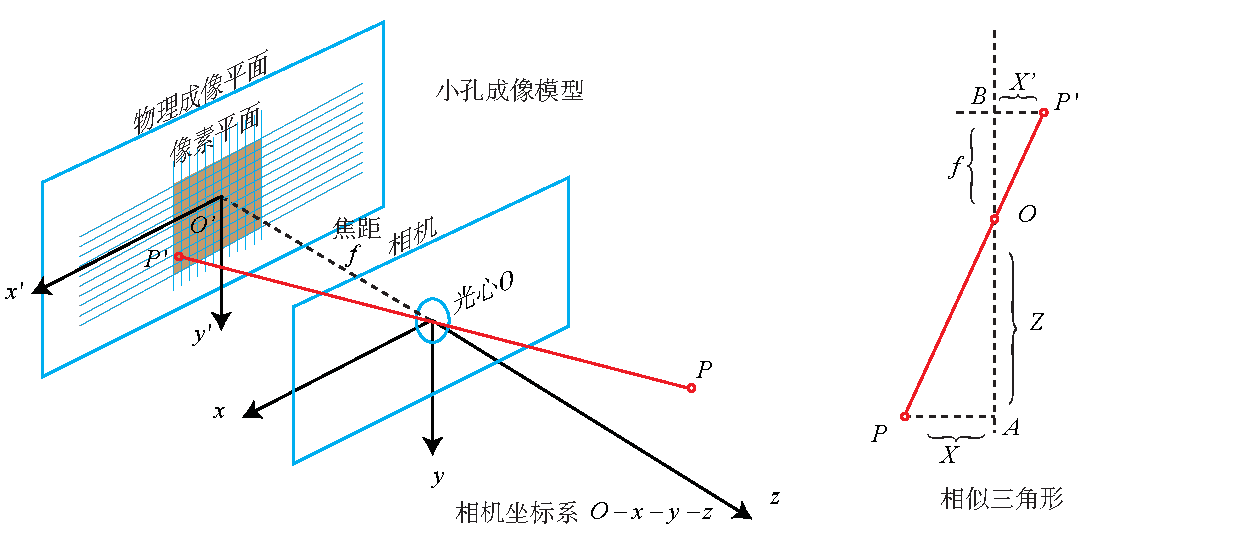
\includegraphics[width=.95\textwidth]{cameraModel/cameraModel.pdf}
	\caption{Pinhole camera model. }
	\label{fig:cameraModel}
\end{figure}

Let's take a look at the simple geometry in this model. Let $O-x-y-z$ be the camera coordinate system. Commonly we put the $z$ axis to the front of the camera, $x$ to the right, and $y$ to the down (so in this figure we should stand on the left side to see the right side). $O$ is the camera's \textbf{Optical Center}, which is also the ``hole'' in the pinhole model. The 3D point $P$, after being projected through the hole $O$, falls on the physical imaging plane $O'-x'-y'$, and produce the image point $P'$. Let the coordinates of $P$ be $[X,Y,Z]^\mathrm{T}$, $P'$ is $[X',Y',Z']^\mathrm{T}$, and set the physical distance from the imaging plane to camera plane is $f$ (focal length). Then, according to the similarity of the triangles, there are:
\begin{equation}
\frac{Z}{f} = -\frac{X}{{X'}} =-\frac{Y}{{Y'}}.
\end{equation}
The negative sign indicates that the image is inverted. However, the image obtained by the actual camera is not an inverted image (otherwise the usage of the camera would be very inconvenient). In order to make the model more realistic, we can equivalently place the imaging plane symmetrically in front of the camera, along with the 3D space points on the same side of the camera coordinate system, as shown by \autoref{fig:planes}. This can remove the negative sign in the formula to make the formula more compact:

\begin{equation}
\frac{Z}{f} = \frac{X}{{X'}} =\frac{Y}{{Y'}}.
\end{equation}

\begin{figure}[!htp]
	\centering
	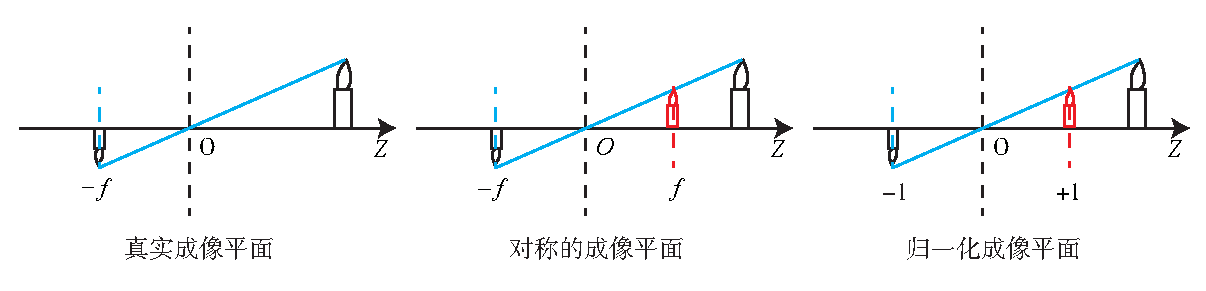
\includegraphics[width=1.0\textwidth]{cameraModel/planes.pdf}
	\caption{The real, symmetric and normalized image plane.}
	\label{fig:planes}
\end{figure}

Put $X', Y'$ to the left side:
\begin{equation}\label{eq:P2Pprime}
\begin{array}{l}
X' = f\frac{X}{Z}\\
Y' = f\frac{Y}{Z}
\end{array}.
\end{equation}

Readers may ask why can we seem to arbitrarily move the imaging plane to the front? In fact this is just a mathematical approach to handle the camera projection, and most of the images captured by the camera are not upside-down - the camera's software will flip the image for you, so what we actually get is the image on the symmetric plane. So, although from the physical principle, the pin-hold image should be inverted, but since we have pre-processed the image, it is not bad to take the symmetric one. Therefore, without causing ambiguity, we often emit the minus symbol in the pinhole model.

The formula~\eqref{eq:P2Pprime} describes the spatial relationship between the point $P$ and its image, where the units of all points are meters,  for example, a focal length may be 0.2 meters and $X'$ be 0.14 meters. However, in the camera, we end up with pixels, where we need to sample and quantize the pixels on the imaging plane. In order to describe the process by which the sensor converts the perceived light into image pixels, we set a pixel plane $o-u-v$ fixed on the physical imaging plane. Finally, we get \textbf{pixel coordinates} of $P'$ in the pixel plane: $[u,v]^\mathrm{T}$.

The usual definition ot the \textbf{pixel coordinate system}\footnote{ Or image coordinate system, see section 2 of this lecture. } is : the origin $o'$ is in the upper left corner of the image, the $u$ axis is parallel to the $x$ axis, and the $v$ axis is parallel to the $y$ axis. Between the pixel coordinate system and the imaging plane, there is an obvious \textbf{zoom} and a \textbf{translation of the origin}. We set the pixel coordinates to scale $\alpha$ times on the $u$ axis and $\beta$ times on $v$. At the same time, the origin is translated by $[c_x, c_y]^\mathrm{T}$. Then, the relationship between the coordinates of $P'$ and the pixel coordinate $[u,v]^\mathrm{T}$ is:
\begin{equation}
\label{eq:project2pixel1} 
\left\{
\begin{matrix} 
u=\alpha X' + c_x\\ 
v=\beta Y' + c_y
\end{matrix}
\right. .
\end{equation}

Put it into~\eqref{eq:P2Pprime} and set $\alpha f$ as $f_x$, $\beta f$ as $f_y$:
\begin{equation}
\left\{
\begin{matrix} 
u=f_x\frac{X}{Z} + c_x\\ 
v=f_y\frac{Y}{Z} + c_y
\end{matrix}
\right. ,
\end{equation}
where $f$ is the focal length in meters, $\alpha, and \beta$ is in pixels/meter, so $f_x, f_y$ and $c_x, c_y$ are in pixels. It would be more compact to write this form as a matrix, but we need to use homogeneous coordinates on the left and non-homogeneous coordinates on the right:
\begin{equation}
\label{eq:intrinmatrix} 
\begin{pmatrix} u\\ v\\ 1 \end{pmatrix}=\frac{1}{Z}\begin{pmatrix} f_x & 0&c_x \\ 0& f_y& c_y\\ 0&0 & 1 \end{pmatrix}\begin{pmatrix} X\\ Y\\ Z \end{pmatrix} 
\buildrel \Delta \over =\frac{1}{Z} \mathbf{K} \mathbf{P}.
\end{equation}

Let put $Z$ to the left side as in most books:
\begin{equation}
Z \begin{pmatrix} u\\ v\\ 1 \end{pmatrix}= \begin{pmatrix} f_x & 0&c_x \\ 0& f_y& c_y\\ 0&0 & 1 \end{pmatrix}\begin{pmatrix} X\\ Y\\ Z \end{pmatrix} 
\buildrel \Delta \over = \mathbf{K} \mathbf{P}.
\end{equation}

In this equation, we refer to the matrix composed of the middle quantities as the camera's \textbf{inner parameter matrix} (o Intrinsics)$\mathbf{K}$. It is generally believed that the internal parameters of the camera are fixed after manufacturing and will not change during usage. Some camera manufacturers will tell you the internal parameters of the camera, and sometimes you need to estimate the internal parameters by yourself, which is called \textbf{calibration}. In view of the maturity of the calibration algorithm (such as the famous Zhang Zhengyou's calibration \textsuperscript{\cite{Zhang1999}}), it will not be introduced here \footnote{I'm sure professor Zhang has a copy of this book now.}. 

There are internal parameters, and naturally there must be something like ``external parameters''. In the equation ~\eqref{eq:intrinmatrix}~, we use the coordinates of $P$ in the camera coordinate system, but in fact the  coordinates of $P$ should be its world coordinates because the camera is moving (we use symbol $\mathbf{P}_w$). It should be converted to the camera coordinate system based on the current pose of the camera. The pose of the camera is described by its rotation matrix $\mathbf{R}$ and the translation vector $\mathbf{t}$. Then there are:

\begin{equation}
\label{eq:cameraprojection}
Z \mathbf{P}_{uv}=
Z \left[ \begin{array}{l}
u\\
v\\
1
\end{array} \right] = \mathbf{K} \left( {\mathbf{R}{ \mathbf{P}_w} + \mathbf{t}} \right) =  \mathbf{K} \mathbf{T} \mathbf{P}_w .
\end{equation}

Note that the latter formula implies a conversion from homogeneous to non-homogeneous coordinates (can you see it?)\footnote{We use homogeneous coordinates in $\mathbf{T}\mathbf{P}$, then convert to non-homogeneous coordinates, and then multiply it by $\mathbf{K}$. }. It describes the projection relationship of world coordinates to pixel coordinates of $P$. Among them, the camera's pose $\mathbf{R}, \mathbf{t}$ is also called the camera's \textbf{extrinsics} \footnote{In robots or autonomous vehicles, the extrinsics is sometimes explained the transform between the camera coordinate system and the robot body coordinate system, describing ``where the camera is installed''. }. Compared with the intrinsics, the extrinsics may change with the camera installation, and is also the target to be estimated in the SLAM if we only have a camera.

The projection process can also be viewed from another perspective. The formula ~\eqref{eq:cameraprojection} shows that we can convert a world coordinate point to the camera coordinate system first, and then remove the value of its last dimension (that is, the depth of the point from the imaging plane of the camera), which is equivalent to the \textbf{normalization} on the last dimension. By this way we get the projection of the point $P$ on the camera \textbf{normalized plane}:
\begin{equation}
\left( {\mathbf{R}{\mathbf{P}_w} + \mathbf{t}} \right) = \underbrace{\left[ X,Y,Z\right]^\mathrm{T}}_{\text{Camera Coordinates}} \to \underbrace {\left[ {X/Z,Y/Z,1} \right]^\mathrm{T}}_{\text{Normalized Coordinates}}.
\end{equation}

The \textbf{normalized coordinates} can be seen as a point in the $z=1$ plane in front of the camera\footnote{Note that in the actual calculation, it is necessary to check whether $Z$ is positive, because the negative $Z$ can also get a point on the normalized plane by this method. However, the camera does not capture the scene behind the imaging plane. }.This $z=1$ plane is also called \textbf{normalized plane}. We normalize the coordinates and then multiply it with the intrinsic matrix, yielding the pixel coordinates, so we can also consider the pixel coordinates $[u,v]^\mathrm{T}$ as the result of quantitative measurements on points on the normalized plane. It can also be seen from this model that if the camera coordinates are multiplied by any non-zero constant at the same time, the normalized coordinates are the same, which means that the \textbf{depth is lost during the projection process}, so in monocular vision the depth value of the pixel cannot be obtained by a single image.

\subsection{Distortion}
In order to get a larger FoV (Field-of-View), we normally add a lens in front of the camera. The addition of the lens has an influence on the propagation of light during imaging: (1) the shape of lens may affect the propagation way of light, (2) during the mechanical assembly, the lens and the imaging plane are not completely parallel, which also makes the projected position change.

There are some mathematical models to describe the \textbf{distortion} caused by the shape of the lens. In the pinhole model, a straight line keeps straight when projected onto the pixel plane. However, in real photos, the lens of the camera tends to make a straight line in the real environment become a curve \footnote{Yes, it is no longer straight, but becomes curved. If it makes an inside curve, it is called barrel-like distortion; otherwise if the curve looks outward, it is cushion-like distortion. }. The closer to the edge of the image, the more obvious this phenomenon is. Since the lenses actually produced are often center-symmetrical, this makes the irregular distortion generally radially symmetrical. They fall into two main categories: \textbf{barrel-like distortion} and \textbf{cushion-like distortion}, as shown by \autoref{fig:distortion}.
\begin{figure}[!t]
	\centering
	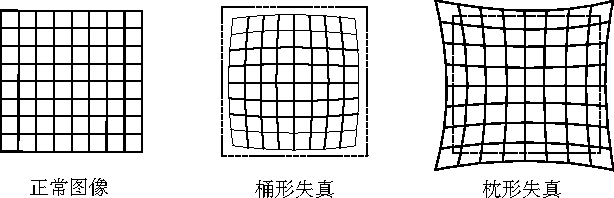
\includegraphics[width=0.7\textwidth]{cameraModel/distortion.pdf}
	\caption{The radical distortion.}
	\label{fig:distortion}
\end{figure}

In barrel distortion the radius of pixels decreases as the distance from the optical axis increases, while the cushion distortion is just the opposite. In both distortions, the line that intersects the intersection of the center of the image and the optical axis remains the same.

In addition to the shape of the lens, which introduces radial distortion, \textbf{tangential distortion} is introduced in during assembly of the camera because the lens and the imaging surface cannot be strictly parallel, as shown by \autoref{fig:tangen}.

\begin{figure}[!t]
	\centering
	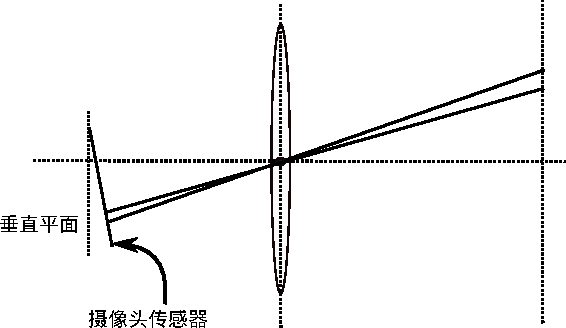
\includegraphics[width=0.7\textwidth]{cameraModel/tangen.pdf}
	\caption{Tangential distortion.}
	\label{fig:tangen}
\end{figure}

To better understand radial and tangential distortion, we describe them in more rigorous mathematical form. Consider any point on the \textbf{normalized plane}, $\mathbf{p}$, whose coordinates are $[x,y]^\mathrm{T}$, or $[r, \theta]^\mathrm{T}$ in the form of polar coordinates, where $r$ represents the distance between the point $\mathbf{p}$ and the origin of the coordinate system, and $\theta$ represents the angle to the horizontal axis. Radial distortion can be seen as a change in the coordinate point along the length, that is, its radius from the origin. Tangential distortion can be seen as a change in the coordinate point along the tangential direction, that is, the horizontal angle has changed. It is generally assumed that these distortions are polynomial, namely:
\begin{equation}
\label{eq:distortion} 
\begin{matrix}
x_\mathrm{distorted} = x(1+k_1r^2+k_2r^4+k_3r^6)\\
y_\mathrm{distorted} = y(1+k_1r^2+k_2r^4+k_3r^6)
\end{matrix},
\end{equation}
where $[x_\mathrm{distorted}, y_\mathrm{distorted}]^\mathrm{T}$ is the \textbf{normalized coordinates} of the point after distortion. On the other hand, for \textbf{tangential distortion}, we can use the other two parameters $p_1,p_2$ to describe it:
\begin{equation}
\label{eq:tangen} 
\begin{matrix}
x_\mathrm{distorted} = x+2p_1xy+p_2(r^2+2x^2)\\
y_\mathrm{distorted} = y+p_1(r^2+2y^2)+2p_2xy
\end{matrix}. 
\end{equation}
Put~\eqref{eq:distortion} and~\eqref{eq:tangen} together we get a joint model with 5 distortion coefficients. The complete form is:
\begin{equation}
\left\{\begin{matrix} x_\mathrm{distorted} =x(1+k_1r^2+k_2r^4+k_3r^6)+2p_1xy+p_2(r^2+2x^2)\\ 
y_\mathrm{distorted} = y(1+k_1r^2+k_2r^4+k_3r^6)+p_1(r^2+2y^2)+2p_2xy
\end{matrix}\right. .
\end{equation}

In the above process of correcting distortion, we used 5 distortion coefficients. In practical applications, you can flexibly choose to number of parameters, for example, only selecting $k_1, p_1, p_2$, or use $k_1, k_2, p_1, p_2$, etc.

In this section, we modeled the camera's imaging process using a pinhole model and described the radial and tangential distortions caused by the lens. In the actual image system, researchers have proposed many other models, such as the affine model and perspective model, and there are many other types of distortion. In most of the visual SLAM systems, pinhole models and rad-tan distortion models are sufficient, so we will not describe other one.

It is worth mentioning that there are two ways of undistortion (or correction). We can choose to undistort the entire image first, get the corrected image, and then discuss the spatial position of the points on the image. Alternatively, we can also discuss some feature points in the distorted image, and find its real position through the distortion equation. Both are feasible, but the former seems to be more common in visual SLAM. Therefore, when an image is undistorted, we can directly establish a projection relationship with the pinhole model without considering distortion. Therefore, in the discussion that follows, we can directly assume that the image has been undistorted.

Finally, let's summarize the imaging process of a monocular camera:

\begin{enumerate}
	\item First, there is a point $P$ in the world coordinate system, and its world coordinates are $\mathbf{P}_w$.
	\item Since the camera is moving, its motion is described by $\mathbf{R}, \mathbf{t}$ or  transform matrix $\mathbf{T} \in \mathrm{SE}(3)$. The camera coordinates for $P$ are $\mathbf{\tilde{P}}_c = \mathbf{R} \mathbf{P}_w + \mathbf{t}$.
	\item The $\mathbf{\tilde{P}}_c$ component is $X,Y,Z$, and they are projected onto the normalized plane $Z=1$ to get the normalized coordinates: $\mathbf{P}_c = [X/Z, Y/Z, 1]^\mathrm{T}$\footnote{Note that $Z$ may be less than 1, indicating that the point is behind the normalization plane and it should not be projected on the camera plane.}.
	\item If the image is distorted, the coordinates of $\mathbf{P}_c$ after distortion are calculated according to the distortion parameters.
	\item Finally, the distorted coordinates of $P$ pass through the intrinsics and we find its pixel coordinates: $\mathbf{P}_{uv} = \mathbf{K} \mathbf{P}_c$.
\end{enumerate}

In summary, we have talked about four coordinates: the world coordinates, the camera coordinates, the normalized coordinates, and the pixel coordinates. Readers should clarify their relationship, which reflects the entire imaging process and will be used in the future.

\subsection{Stereo Cameras}
The pinhole camera model describes the imaging model of a single camera. However, we cannot determine the specific location of a spatial point on by a single pixel. This is because all points on the line from the camera's optical center to the normalized plane can be projected onto that pixel. Only when the depth of $P$ is determined (such as through a binocular or RGB-D camera) can we know exactly its spatial location, as shown in \autoref {fig:pixelLocation}~.

\begin{figure}[!ht]
    \centering
    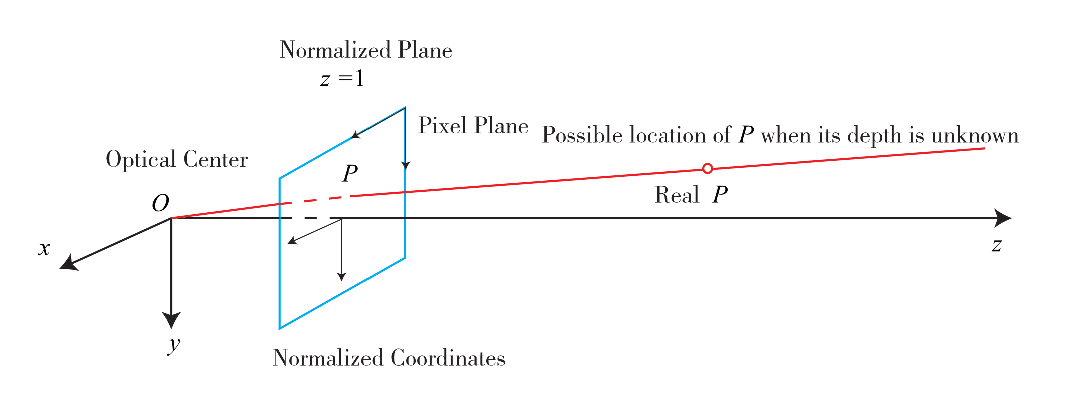
\includegraphics[width=1.0\textwidth]{cameraModel/pixelLocation.pdf}
    \caption{The possible location of a single pixel.}
    \label{fig:pixelLocation}
\end{figure}

There are many ways to measure the pixel distance (or depth). For example, the human eye can judge the distance of the object according to the difference (or parallax) of the scene seen by the left and right eyes. The principle of the binocular camera is also the same: by simultaneously acquiring the images of the left and right cameras, and calculating the parallax/disparity between the images, the depth of each pixel is estimated. In the following paragraph we  briefly describe the imaging principle of the stereo camera (as shown in \autoref{fig:stereoCamera}~).

A binocular camera is generally composed of a left-eye camera and a right-eye camera. Of course, it can also be made up and down, but the mainstream binoculars we've seen are all left and right. In left and right cameras are often regarded as simple pin-hole cameras. They are synchrozied and placed horizontally, meaning that the centers of both cameras are on the same $x$ axis. The distance between the two centers is called \textbf {baseline} (denoted as $b$), which is an important parameter.

\begin{figure}[!ht]
    \centering
    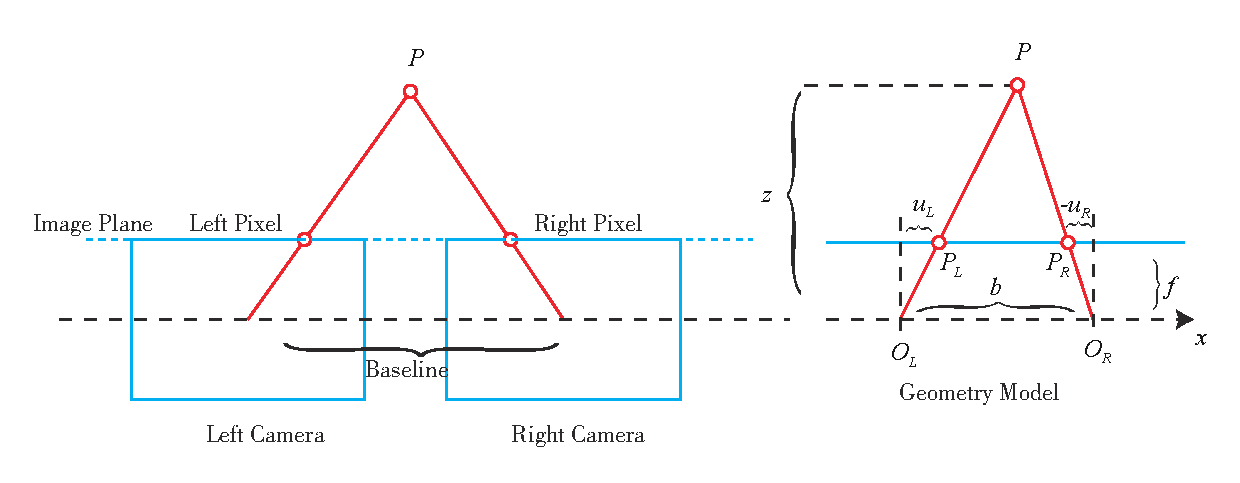
\includegraphics[width=1.0\textwidth]{cameraModel/stereoCamera.pdf}
    \caption{Geometry model of stereo cameras from upside down. The $O_L,O_R$ are left and right optical centers. $f$ is the focal length, $u_L$ and $u_R$ are pixel corrdinates of a same point along $x$ axis. Note that $u_R$ should be a negative value in this figure, so the pysical distance should be $-u_R$.}
    \label{fig:stereoCamera}
\end{figure}

Now consider a 3D point $P$, which is projected into the left-eye and the right-eye, written as $P_L, P_R$. Due to the presence of the camera baseline, these two imaging positions are different. Ideally, since the left and right cameras are only shifted on the $x$ axis, the image of $P$ also differs only on the $x$ axis (corresponding to the $u$ axis of the image). Take the left pixel coordinate as $u_L$ and the right coordinate as $u_R$. The geometric relationship is shown on the right of \autoref{fig:stereoCamera}. According to the similarity relationship between $ \triangle P P_L P_R$ and $\triangle P O_L O_R$, there are:

\begin{equation}
\frac{{z - f}}{z} = \frac{{b - {u_L} + {u_R}}}{b}.
\end{equation}

Rearrangle it and we have:
\begin{equation}
z = \frac{{fb}}{d}, \quad d \buildrel \Delta \over = {u_L} - {u_R},
\end{equation}
where $d$ is defined as the difference between the horizontal coordinates of the left and right figures, and is called \textbf{disparity} or \textbf{parallax}. Based on the parallax, we can estimate the distance between a pixel and the camera. Parallax is inversely proportional to distance: the larger the parallax is, the closer the distance is \footnote {Readers can simulate it with your own eyes.}. At the same time, since the parallax is at least one pixel, there is a theoretical maximum value for the binocular depth, which is determined by $fb$. We see that the in order to see the far away things, we need a larger stereo camera; conversely, small binocular devices can only measure very close distances. By analogy, when the human eye looks at a very distant object (such as a very distant airplane), it is usually impossible to accurately determine its distance.

Although the formula for calculating the depth from parallax is simple, the calculation of parallax $d$ itself is more difficult. We need to know exactly where a pixel of the left-eye image appears in the right-eye image (that is, the corresponding relationship). This also belongs to the kind of task that is ``easy for humans but difficult for computers''. When we want to calculate the depth of each pixel in an image, the calculation amount and accuracy will become a problem, and the parallax can be calculated only in the place where the image texture is rich. Due to the amount of calculation, binocular depth estimation still needs to use GPU or FPGA to make the distance calculation run in real time. This will be mentioned in lecture 13.

\subsection{RGB-D Cameras}
Compared to the binocular camera's way of calculating depth, the RGB-D camera's approach is more ``active'': it can actively measure the depth of each pixel. The current RGB-D cameras can be divided into two categories according to their principle (see \autoref {fig:RGBDCamera} ~):

\begin{enumerate}
\item The first kind of RGB-D sensor uses \textbf{Infrared Structured Light} (Structured Light) to measure pixel distance. Many of the old RGB-D sensors are belong to this kind, for example, the Kinect 1st generation, Project Tango 1st generation, Intel RealSense, etc.
\item The second kind measures pixel distance using the \textbf{Time-of-flight (ToF)}. Examples are Kinect 2 and some existing ToF sensors.
\end{enumerate}

\begin{figure}[!ht]
    \centering
    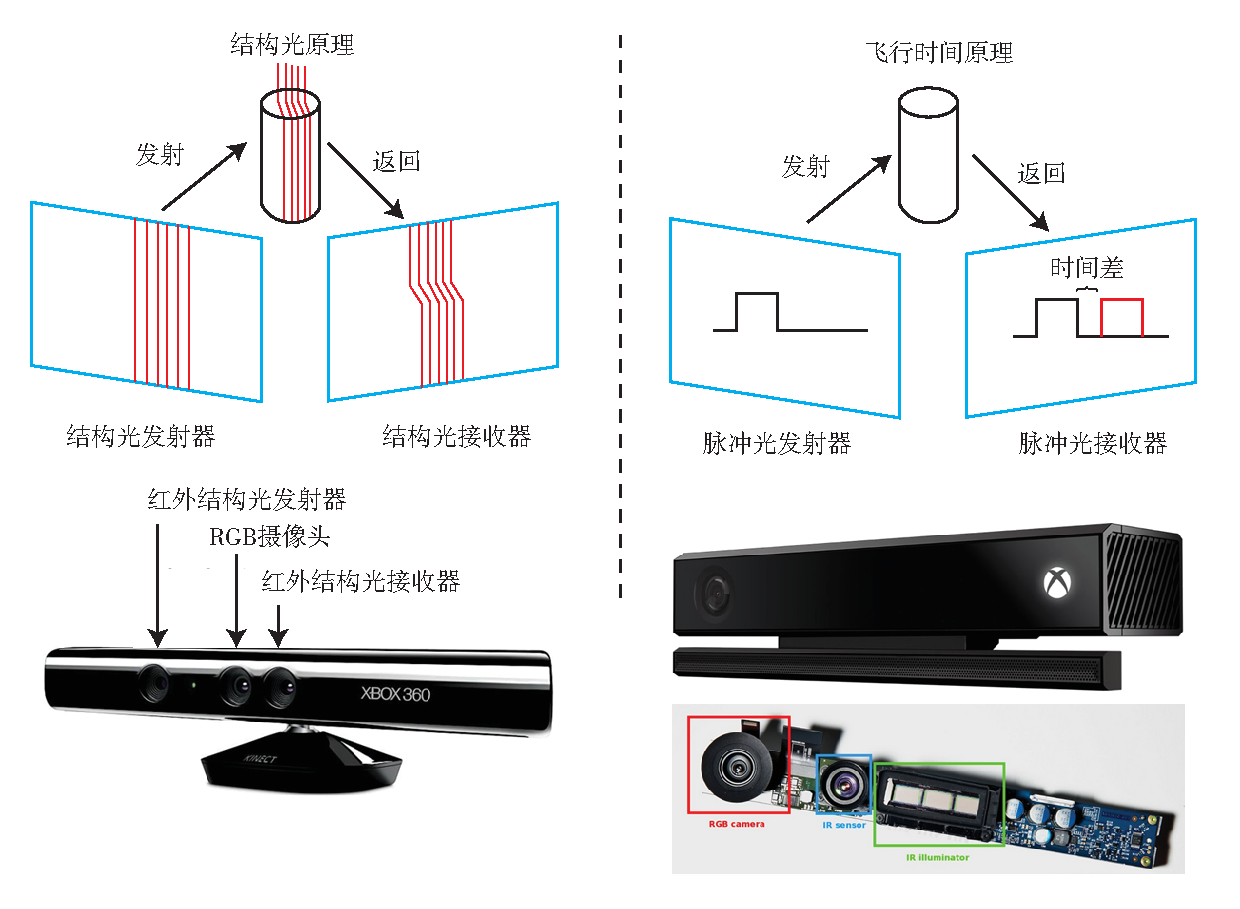
\includegraphics[width=1.0\textwidth]{cameraModel/rgbdCamera.pdf}
    \caption{RGB-D Cameras}
    \label{fig:RGBDCamera}
\end{figure}

Regardless of the type, the RGB-D camera needs to emit a beam of light (usually infrared light) to the target object. In the principle of structured light, the camera calculates the distance between the object and itself based on the returned structured light pattern. In the ToF principle, the camera emits light pulse to the target, and then determines the distance according to the time of flight of the beam. The ToF principle is very similar to the laser sensor, except that the laser obtains the distance by scanning point by point (or line by line), and the ToF camera can obtain the pixel depth of the entire image, which is also the characteristics of the RGB-D camera. So, if you take apart an RGB-D camera, you will usually find that there will be at least one transmitter and one receiver in addition to the ordinary camera.

After measuring the depth, the RGB-D camera usually completes the pairing between the depth and color map pixels according to the position of each camera at the time of production, and outputs a pixel-to-pixel corresponding color image and depth image. We can read the color information and distance information at the same image position, calculate the 3D camera coordinates of the pixels, and generate a point cloud. RGB-D data can be processed either at the image level or the point cloud level. The second experiment of this lecture will demonstrate the point cloud construction of RGB-D cameras.

The RGB-D camera can measure the distance of each pixel in real time. However, due to this measurement of transmitting and receiving, its range of use is limited. RGB-D cameras that use infrared light for depth measurement are susceptible to interference from infrared light emitted by daylight or other sensors, so they cannot be used outdoors. Without modulation, multiple RGB-D cameras can interfere with each other. For transmissive objects, the position of these points cannot be measured because they cannot receive reflected light. In addition, RGB-D cameras have some disadvantages in terms of cost and power consumption.

\section{Images}
Cameras and lens convert the information in the three-dimensional world into a photo composed of pixels, which is then stored in the computer as a data source for subsequent processing. In mathematics, images can be described by a matrix; in computers, they occupy a continuous disk or memory space, which can be represented by a two-dimensional array. In this way, the program does not have to distinguish whether they are dealing with a numerical matrix or a meaningful image.

In this section, we will introduce some basic operations of computer image processing. In particular, we are going to introduce the basic steps of processing images with OpenCV, and lay the foundation for subsequent chapters. Let's start with the simplest case, the grayscale image. In a grayscale image, each pixel position $ (x, y) $ corresponds to a grayscale value of $ I $. Therefore, an image with a width of $ w $ and a height of $ h $ can be mathematically written as a function:
\[
(I) (x, y): \mathbb {R} ^ 2 \mapsto \mathbb {R},
\]
where $ (x, y) $ is the coordinate of the pixel. However, computers cannot express real space, so we need to quantify the subscripts and image readings within a certain range. For example, $ x, y $ are usually integers starting with 0 to $w-1, h-1$. In common grayscale images, an integer of $0 \textasciitilde 255$ (that is, an unsigned char in C++, 1 byte) is used to express the grayscale reading of the image. Then, a grayscale image with a width of 640 pixels and a height of 480 pixels can be expressed as:
\begin{lstlisting}[language=C++, caption=Use 2D array to express an image]
unsigned char image[480][640];
\end{lstlisting}

Why does the two-dimensional array here has the size of 480 $ \times $ 640? Because in the program, the first index of 2D array is the row, and the second index is the column. In an image, the number of rows (or the $y$ axis) in the array corresponds to the height of the image, and the number of columns (or the $x$ axis) corresponds to the width of the image.
\begin{figure}[!t]
    \centering
    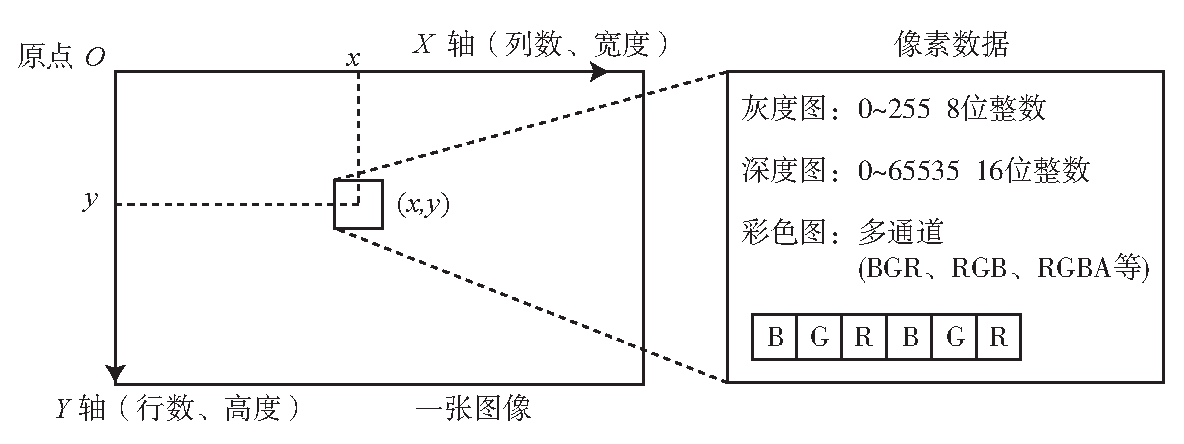
\includegraphics[width=0.84\textwidth]{cameraModel/image.pdf}
    \caption{Pixels in an image.}
    \label{fig:imagesInComputer}
\end{figure}

Let's examine the content of this image. Images are naturally made up of pixels. When accessing a certain pixel, you need to specify its coordinates, as shown in \autoref{fig:imagesInComputer}~. The left side of the figure shows how the traditional pixel coordinate system is defined. The origin is in the upper left corner of the image, $X$ axis is from left to right, and $Y$ is top-down. If it has a third axis, the $ Z $ axis, then according to the right-hand rule, the $ Z $ axis should be from outside to inside (or front in 3D space). This definition is consistent with the camera coordinate system. The width or number of columns of an image corresponds to the $ X $ axis; the number of rows, or the height of an image corresponds to its $ Y $ axis.

According to this definition, if we discuss a pixel located at $x,y$, then the code of accessing its memory in computer should be:
\begin{lstlisting}[language = C++, caption = Accessing image pixels]
unsigned char pixel = image[y][x];
\end{lstlisting}

It corresponds to the reading of the gray value $ I(x,y) $. Please note the order of $ x $ and $ y $ here. Although we tirelessly discuss the problem of coordinate systems, errors like this index sequence will still be one of the most common errors encountered by novices during debugging. If you accidentally change the coordinates of $ x, y $ when writing a program, the compiler cannot provide any useful information, and all you can see is a segment fault in runtime.

The gray scale of a pixel can be recorded as an 8-bit unsigned integer, which is a value of 0\textasciitilde 255. If we have more information to record, one byte is probably not enough. For example, in the depth map of an RGB-D camera, the distance between each pixel is recorded. This distance is usually measured in millimeters, and the range of RGB-D cameras is usually around a dozen meters, exceeding 255. At this time, people will use 16-bit integers (unsigned short in C++) to record the depth map information, that is, the value at 0\textasciitilde 65535. When converted to meters, it can represent up to 65 meters, which is enough for RGB-D cameras.

The representation of a color image requires the concept of a channel. In computers, we use a combination of three colors: red, green, and blue to express any color. Therefore, for each pixel, three values ​​of R, G, and B are recorded, and each value is called a channel. For example, the most common color image has three channels, each of which is represented by an 8-bit integer. Under this rule, one pixel occupies 24-bit space.

The number and order of channels can be freely defined. In OpenCV color images, the default order of channels is B, G, R. That is, when we get a 24-bit pixel, the first 8 bits represent the blue value, the middle 8 bits represent the green value, and the last 8 bits represent the red value. In the same way, the order of R, G, and B can also be used to represent a color image. If you want to express the transparency of the image, use R, G, B, A four channels.

\section{Practice: Images in Computer Vision}
\subsection{Basic Usage of OpenCV}
The following is a demo program to understand how to access the image in OpenCV, and how to visit its pixels.

\subsubsection{Install OpenCV}
OpenCV \footnote {Official homepage: \url{http://opencv.org}. } provides a large number of open source image algorithms, and is a very widely used image processing algorithm library in computer vision. This book also uses OpenCV for basic image processing. Before using, readers must install it from library or from source code. Under Ubuntu, there are two options: \textbf{install from source code} or \textbf {only install binary library files}:

\begin{enumerate}
\item Install from source means to download all OpenCV source code from the OpenCV website, compile and install on the machine for usage. The advantage is that you can freely choose which version to install, and the source code is accessible, but it takes some compilation time.
\item Or, we can only installs the binary library file, which means it was pre-compiled by the Ubuntu community, so that there is no need to recompile it.
\end{enumerate}

Since we use a newer version of OpenCV, we must install it from the source code. First, you can adjust some compilation options to match the programming environment (for example, whether you need GPU acceleration, etc.); furthermore, from the source code installation we can use some additional functions. OpenCV currently maintains two major versions, divided into OpenCV 2.4 series and OpenCV 3 series \footnote{In 2020 we can also use version 4.0 or higher.}. This book uses the OpenCV \textbf {3} series.

Because the OpenCV project is relatively large, it will not be placed under 3rdparty in this book. Readers can download it from ~ \url{http://opencv.org/downloads.html}~ and select the OpenCV for Linux version. You will get a compressed package like opencv-3.1.0.zip. Unzip it to any directory, we found that OpenCV is also a CMake project.

Before compiling, first install the dependencies of OpenCV:
\begin{lstlisting}[language=sh, caption=Terminal input:]
sudo apt-get install build-essential libgtk2.0-dev libvtk5-dev libjpeg-dev libtiff4-dev libjasper-dev libopenexr-dev libtbb-dev
\end{lstlisting}

In fact, OpenCV has many dependencies, and the lack of certain compilation items will affect some of its functions (but we will not use all the functions). OpenCV will check whether the dependencies will be installed during CMake and adjust its own functions. If you have a GPU on your computer and the relevant dependencies are installed, OpenCV will also enable GPU acceleration. But for this book, the above dependencies are sufficient.

Subsequent compilation and installation are the same as ordinary CMake projects. After make, please call ``sudo make install'' to install OpenCV on your machine (instead of just compiling it). Depending on the machine configuration, this compilation process may take from 20 minutes to an hour. If your CPU is powerful, you can use commands like ``make -j4'' to call multiple threads to compile (the parameter after -j is the number of threads used). After installation, OpenCV is stored in the /usr/local directory by default. You can look for the installation location of OpenCV header files and library files to see where they are. In addition, if you have installed the OpenCV 2 series before, it is recommended that you install OpenCV 3 elsewhere (think about how this should be done).

\subsection{Basic OpenCV Images Operations}
Now let's go through the basic image operations in OpenCV from a simple example.

\begin{lstlisting}[language=C++,caption=slambook/ch5/imageBasics/imageBasics.cpp]
#include <iostream>
#include <chrono>

using namespace std;

#include <opencv2/core/core.hpp>
#include <opencv2/highgui/highgui.hpp>

int main(int argc, char **argv) {
    // Read the image in argv[1]
    cv::Mat image;
    image = cv::imread(argv[1]); // call cv::imread to read the image from file
    
    // check the data is correctly loaded
    if (image.data == nullptr) { // maybe the file does not exist
        cerr << "file" << argv[1] << " not exist." << endl;
        return 0;
    }
    
    // print some basic information
    cout << "Image cols: " << image.cols << ", rows: " << image.rows 
    << ", channels: " << image.channels() << endl;
    cv::imshow("image", image);      // use cv::imshow to show the image
    cv::waitKey(0);                  // display and wait for a keyboard input
    
    // check image type
    if (image.type() != CV_8UC1 && image.type() != CV_8UC3) {
        // we need grayscale image or RGB image
        cout << "image type incorrect." << endl;
        return 0;
    }
    
    // check hte pixels
    chrono::steady_clock::time_point t1 = chrono::steady_clock::now();
    for (size_t y = 0; y < image.rows; y++) {
        // use cv::Mat::ptr to get the pointer of each row
        unsigned char *row_ptr = image.ptr<unsigned char>(y);  // row_ptr is the pointer to y-th row
        for (size_t x = 0; x < image.cols; x++) {
            // read the pixel on (x,y), x=column, y=row
            unsigned char *data_ptr = &row_ptr[x * image.channels()]; // data_ptr is the pointer to (x,y)
            // visit the pixel in each channel
            for (int c = 0; c != image.channels(); c++) {
                unsigned char data = data_ptr[c]; // data should be pixel of I(x,y) in c-th channel
            }
        }
    }
    chrono::steady_clock::time_point t2 = chrono::steady_clock::now();
    chrono::duration<double> time_used = chrono::duration_cast < chrono::duration < double >> (t2 - t1);
    cout << "time used: " << time_used.count() << " seconds." << endl;
    
    // copying cv::Mat
    // operator = will not copy the image data, but only the reference
    cv::Mat image_another = image;
    // changing image_another will also change image 
    image_another(cv::Rect(0, 0, 100, 100)).setTo(0); // set top-left 100*100 block to zero
    cv::imshow("image", image);
    cv::waitKey(0);
    
    // use cv::Mat::clone to actually clone the data
    cv::Mat image_clone = image.clone();
    image_clone(cv::Rect(0, 0, 100, 100)).setTo(255);
    cv::imshow("image", image);
    cv::imshow("image_clone", image_clone);
    cv::waitKey(0);
    
    // We are not going to copy the OpenCV's documentation here
    // please take a look at it for other image operations like clipping, rotating and scaling.
    
    cv::destroyAllWindows();
    return 0;
}
\end{lstlisting}

In this example, we demonstrated the following operations: image reading, displaying, pixel vising, copying, assignment, etc. When compiling the program, you need to add the OpenCV header file in your ``CMakeLists.txt'', and then link the program to the OpenVC's library. At the same time, due to the use of C ++ 11 standards (such as nullptr and chrono), you also need to set up the c++ standard in compiler flag:

\begin{lstlisting}[language=Python,caption=slambook/ch5/imageBasics/CMakeLists.txt]
# use c++11 standard
set( CMAKE_CXX_FLAGS "-std=c++11" )

# find OpenCV
find_package( OpenCV REQUIRED )
# include its headers
include_directories( ${OpenCV_INCLUDE_DIRS} )

add_executable( imageBasics imageBasics.cpp )

# link the exe to opencv's libs
target_link_libraries( imageBasics ${OpenCV_LIBS} )
\end{lstlisting}

Let's give some notes for the code:
\begin{enumerate}
\item The program reads the image position from argv[1], the first parameter on the command line. We prepared an image (ubuntu.png, an Ubuntu wallpaper, I hope you like it) for readers to test. Therefore, after compilation, use the following command to call this program:
\begin{lstlisting}[language=sh, caption=Terminal input:]
./build/imageBasics ubuntu.png
\end{lstlisting}
If you call this program in the IDE, be sure to give it parameters at the same time. This can be configured in the launch configuration dialog if you are using Clion.
\item In line 10 \textasciitilde to 18, use the cv::imread function to read the image, and display the image and basic information.
\item In line 35 \textasciitilde 46, we iterate over all pixels in the image and calculates the time spent in the entire loop. Please note that the pixel visiting method is not unique, and the method given by the example is not the most efficient way. OpenCV provides an iterator of cv::Mat, you can traverse the pixels of the image through the iterator. Or, cv::Mat::data provides a raw pointer to the beginning of the image data, you can directly calculate the offset through this pointer, and then get the actual memory location of the pixel. The method used in the example is to facilitate the reader to understand the structure of the image.

On the author's machine (virtual machine), it takes about 12.74ms to traverse this image. You can compare the speed on your machine. However, we are using the default debug mode of CMake, which is much slower than the release mode.

\item OpenCV provides many functions for manipulating images, we will not list them one by one, otherwise this book will become an OpenCV operation manual. The example shows the most common things like image reading and displaying, as well as the deep copy function in cv::Mat. During the programming process, readers will also encounter operations such as image rotation and interpolation. At this time, you should refer to the corresponding documentation of the function to understand their principles and usage.
\end{enumerate}

It should be noted that OpenCV is not the only image library, it is just one of the more widely used one. However, most image libraries have the similar image operations. We hope that readers can understand the representation of images in other libraries after understanding the representation of images in OpenCV, so that they can quickly adjust to any other libraries. In addition, since cv::Mat is also a matrix class, in addition to representing images, we can also use it to store matrix data such as rotation matrix. But it is generally believed that Eigen is more efficient for use with fixed-size matrices.

\subsection{Image Undistortion}
We've introduced the rad-tan distortion model in previous section, now let write an example to show the implementation. OpenCV has provided the cv::Undistort function for us, but we will also give a hand-written undistortion function to show the principles.

\begin{lstlisting}[language=C++,caption=slambook/ch5/imageBasics/undistortImage.cpp]
#include <opencv2/opencv.hpp>
#include <string>
using namespace std;
string image_file = "./distorted.png";   // the distorted image 

int main(int argc, char **argv) {
    // In thie program we implement the undistortion by ourselves rather than using opencv
    // rad-tan model params
    double k1 = -0.28340811, k2 = 0.07395907, p1 = 0.00019359, p2 = 1.76187114e-05;
    // intrinsics
    double fx = 458.654, fy = 457.296, cx = 367.215, cy = 248.375;
    
    cv::Mat image = cv::imread(image_file, 0);   // the image type is CV_8UC1
    int rows = image.rows, cols = image.cols;
    cv::Mat image_undistort = cv::Mat(rows, cols, CV_8UC1);   // the undistorted image
    
    // computate the pixels in the undistorted one
    for (int v = 0; v < rows; v++) {
        for (int u = 0; u < cols; u++) {
            // note we are computing the pixel of (u,v) in the undistorted image
            // according to the rad-tan model, compute the coordinates in the distorted image
            double x = (u - cx) / fx, y = (v - cy) / fy;
            double r = sqrt(x * x + y * y);
            double x_distorted = x * (1 + k1 * r * r + k2 * r * r * r * r) + 2 * p1 * x * y + p2 * (r * r + 2 * x * x);
            double y_distorted = y * (1 + k1 * r * r + k2 * r * r * r * r) + p1 * (r * r + 2 * y * y) + 2 * p2 * x * y;
            double u_distorted = fx * x_distorted + cx;
            double v_distorted = fy * y_distorted + cy;
            
            // check if the pixel is in the image boarder
            if (u_distorted >= 0 && v_distorted >= 0 && u_distorted < cols && v_distorted < rows) {
                image_undistort.at<uchar>(v, u) = image.at<uchar>((int) v_distorted, (int) u_distorted);
            } else {
                image_undistort.at<uchar>(v, u) = 0;
            }
        }
    }
    
    // show the undistorted image
    cv::imshow("distorted", image);
    cv::imshow("undistorted", image_undistort);
    cv::waitKey();
    return 0;
}
\end{lstlisting}

Please check the difference between two images by yourself.

\section{Practice: 3D Vision}
\subsection{Stereo Vision}
We have introduced the imaging principle of stereo vision. Now we start from the left and right images, calculate the disparity map corresponding to the left eye, and then calculate the coordinates of each pixel in the camera coordinate system, which will form a \textbf{point cloud}. We have prepared left and right images for the readers, as shown in \autoref {fig:stereoExample}. The following code demonstrates the calculation of disparity map and point cloud:

\begin{lstlisting}[language=C++,caption=slambook/ch5/stereoVision/stereoVision.cpp (Part)]
int main(int argc, char **argv) {
    // intrinsics
    double fx = 718.856, fy = 718.856, cx = 607.1928, cy = 185.2157;
    // baseline
    double b = 0.573;
    
    cv::Mat left = cv::imread(left_file, 0);
    cv::Mat right = cv::imread(right_file, 0);
    cv::Ptr<cv::StereoSGBM> sgbm = cv::StereoSGBM::create(
        0, 96, 9, 8 * 9 * 9, 32 * 9 * 9, 1, 63, 10, 100, 32);    // SGBM is senstive to parameters
    cv::Mat disparity_sgbm, disparity;
    sgbm->compute(left, right, disparity_sgbm);
    disparity_sgbm.convertTo(disparity, CV_32F, 1.0 / 16.0f);
    
    // compute the point cloud
    vector<Vector4d, Eigen::aligned_allocator<Vector4d>> pointcloud;
    
    // change v++ and u++ to v+=2, u+=2 if your machine is slow to get a sparser cloud
    for (int v = 0; v < left.rows; v++)
    for (int u = 0; u < left.cols; u++) {
        if (disparity.at<float>(v, u) <= 10.0 || disparity.at<float>(v, u) >= 96.0) continue;
        
        Vector4d point(0, 0, 0, left.at<uchar>(v, u) / 255.0); // the first three dimensions are xyz, the 4-th is the color
        
        // compute the depth from disparity
        double x = (u - cx) / fx;
        double y = (v - cy) / fy;
        double depth = fx * b / (disparity.at<float>(v, u));
        point[0] = x * depth;
        point[1] = y * depth;
        point[2] = depth;
        
        pointcloud.push_back(point);
    }
    
    cv::imshow("disparity", disparity / 96.0);
    cv::waitKey(0);
    
    // show the point cloud in pangolin
    showPointCloud(pointcloud);
    return 0;
}
\end{lstlisting}

\begin{figure}[!t]
    \centering
    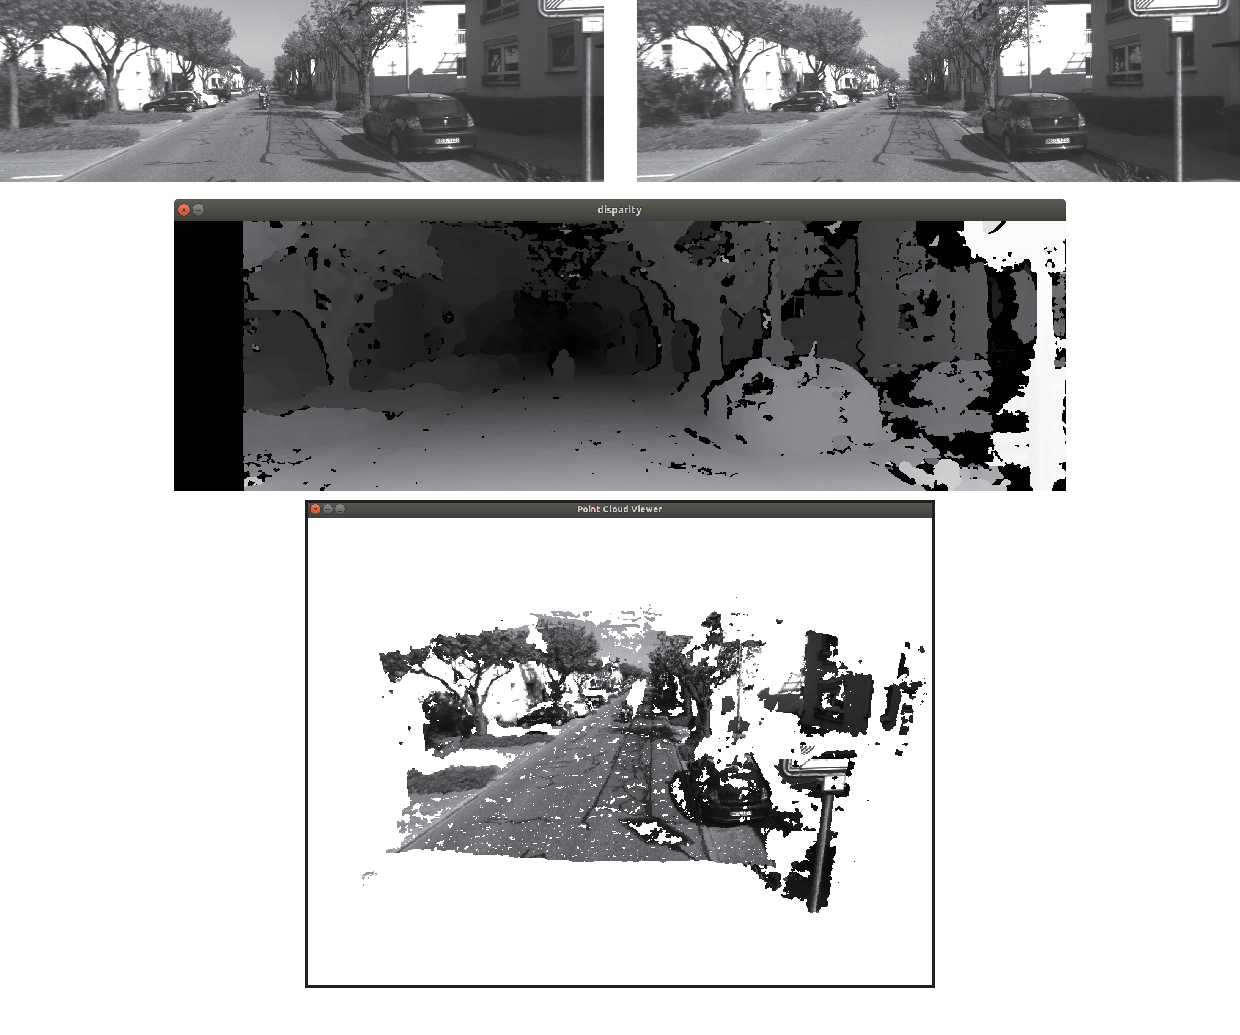
\includegraphics[width=0.9\textwidth]{cameraModel/stereoExample.pdf}
    \caption{Stereo image example. Top-left: left image, top-right: right image, mid: SGBM disparity map, bottom: point cloud. Note that since some of the pixels in the left image is not seen in the right one, so the disparity map will have some empty values.}
    \label{fig:stereoExample}
\end{figure}

In this example, we call the SGBM (Semi-global Batch Matching) \textsuperscript{\cite{Hirschmuller2008}} algorithm implemented by OpenCV to calculate the disparity of the left and right images, and then transform it into the 3D space of the camera through the geometric model of the binocular camera. We use a classic parameter configuration from the internet, and we mainly adjust the maximum and minimum disparity. The disparity data combined with the camera's internal parameters and baseline can determine the position of each point in three-dimensional space. We omit the code related to displaying the point cloud to save some space.

This book is not going to introduce the disparity calculation algorithm of the binocular camera. Interested readers can read the relevant references \textsuperscript{\cite{Scharstein2002, Seitz2006}}. In addition to the binocular algorithm implemented by OpenCV, there are many other libraries focused on achieving efficient parallax calculations. It is still an active and complex subject today.

\subsection{RGB-D Vision}
\label{sec:join-point-cloud}
Finally, we demonstrate an example of RGB-D vision. The convenience of RGB-D cameras is that they can obtain pixel depth information through physical methods. If the internal and external parameters of the camera are known, we can calculate the position of any pixel in the world coordinate system, thereby creating a point cloud map. Now let's demonstrate how to do it.

We have prepared 5 pairs of images, located in the slambook2/ch5/rgbd folder. There are 5 RGB images from 1.png to 5.png under the color/ directory, and 5 corresponding depth images under the depth/. At the same time, the ``pose.txt'' file gives the camera poses of the 5 images (in the form of $ \mathbf{T}_\mathrm{wc} $). The form of the pose record is the same as before, with the translation vector plus a rotation quaternion:
\[
[x, y, z, q_x, q_y, q_z, q_w],
\]
where $q_w$ is the real part of the quaternion. For example, the parameters of the first pair of image are:
\[
[-0.228993, 0.00645704, 0.0287837, -0.0004327, -0.113131, -0.0326832, 0.993042].
\]

Below we write a program to accomplish two things: (1). Calculate the point cloud corresponding to each pair of RGB-D images based on internal parameters; (2). According to the camera pose of each image (that is, external parameters), put the points to a global cloud by the camera poses.

\begin{lstlisting}[language=C++,caption=slambook/ch5/rgbd/jointMap.cpp (Part)]
int main(int argc, char **argv) {
    vector<cv::Mat> colorImgs, depthImgs;
    TrajectoryType poses;         // camera poses
    
    ifstream fin("./pose.txt");
    if (!fin) {
        cerr << "Please run the program in the directory that has pose.txt" << endl;
        return 1;
    }
    
    for (int i = 0; i < 5; i++) {
        boost::format fmt("./%s/%d.%s"); // the image format
        colorImgs.push_back(cv::imread((fmt % "color" % (i + 1) % "png").str()));
        depthImgs.push_back(cv::imread((fmt % "depth" % (i + 1) % "pgm").str(), -1)); // use -1 flag to load the depth image
        
        double data[7] = {0};
        for (auto &d:data) fin >> d;
        Sophus::SE3d pose(Eigen::Quaterniond(data[6], data[3], data[4], data[5]),
        Eigen::Vector3d(data[0], data[1], data[2]));
        poses.push_back(pose);
    }
    
    // compute the point cloud using camera intrinsics
    double cx = 325.5;
    double cy = 253.5;
    double fx = 518.0;
    double fy = 519.0;
    double depthScale = 1000.0;
    vector<Vector6d, Eigen::aligned_allocator<Vector6d>> pointcloud;
    pointcloud.reserve(1000000);
    
    for (int i = 0; i < 5; i++) {
        cout << "Converting RGBD images " << i + 1 << endl;
        cv::Mat color = colorImgs[i];
        cv::Mat depth = depthImgs[i];
        Sophus::SE3d T = poses[i];
        for (int v = 0; v < color.rows; v++)
        for (int u = 0; u < color.cols; u++) {
            unsigned int d = depth.ptr<unsigned short>(v)[u]; // depth value is 16-bit
            if (d == 0) continue; // 0 means no valid value
            Eigen::Vector3d point;
            point[2] = double(d) / depthScale;
            point[0] = (u - cx) * point[2] / fx;
            point[1] = (v - cy) * point[2] / fy;
            Eigen::Vector3d pointWorld = T * point;
            
            Vector6d p;
            p.head<3>() = pointWorld;
            p[5] = color.data[v * color.step + u * color.channels()];   // blue
            p[4] = color.data[v * color.step + u * color.channels() + 1]; // green
            p[3] = color.data[v * color.step + u * color.channels() + 2]; // red
            pointcloud.push_back(p);
        }
    }
    
    cout << "global point cloud has " << pointcloud.size() << " points." << endl;
    showPointCloud(pointcloud);
    return 0;
}
\end{lstlisting}

We can see the point cloud in Pangolin after building it (see \autoref{fig:pointcloudmapping}). 

\begin{figure}[!t]
    \centering
    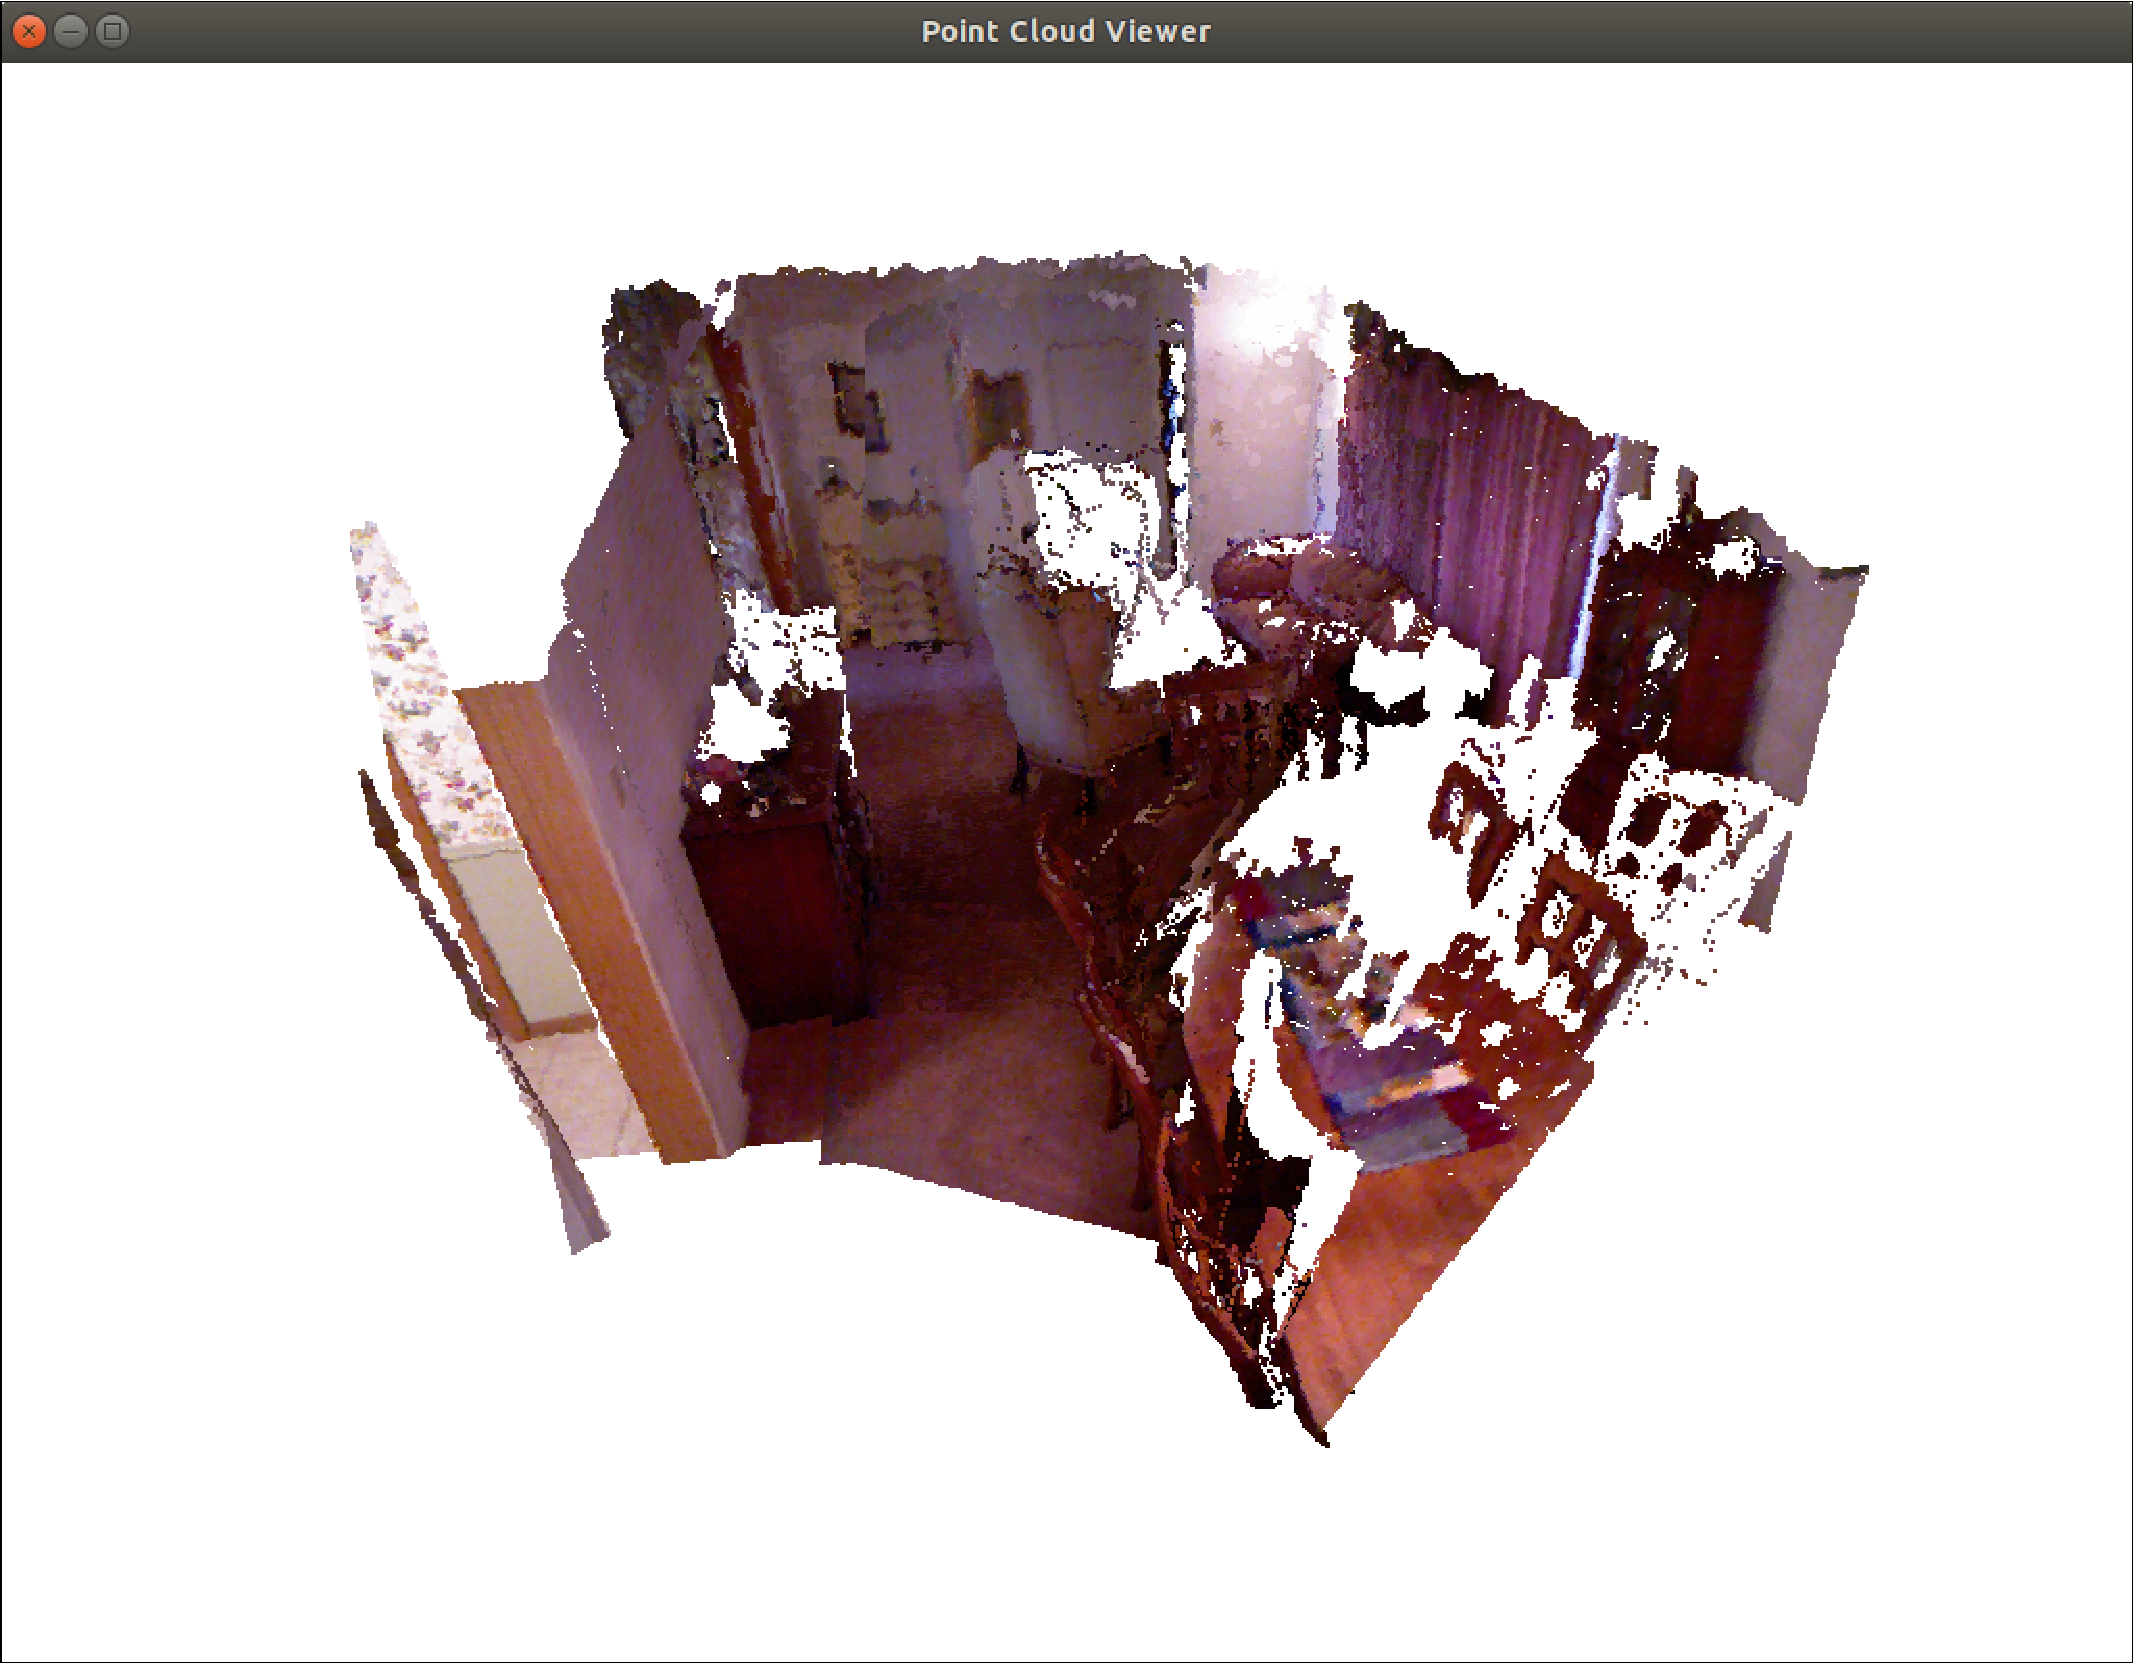
\includegraphics[width=1.0\textwidth]{cameraModel/pointcloud.pdf}
    \caption{See the global point cloud by 5 RGBD image pairs.}
    \label{fig:pointcloudmapping}
\end{figure}

Through these examples, we demonstrated some common monocular, binocular, and depth camera algorithms in computer vision. We hope readers can understand the meaning of the intrinsics, extrinsics and distortion model through these simple examples.

\section * {Exercise}
\begin{enumerate}
\item[\optional] Find a camera (use the camera of your mobile phone or laptop if you don't have one) and calibrate its internal parameters You may use a calibration board, or print out a checkerboard for calibration.
\item Describes the physical meaning of the camera's intrinsics. If the resolution of a camera is doubled and the rest is unchanged, how does its intrinsics change?
\item Search for the calibration method of special cameras (fisheye or panoramic cameras). Where are the differences between them and the pinhole models? 
\item Investigate the similarities and differences between a global shutter camera and a rolling shutter camera. What are their advantages and disadvantages in SLAM?
\item How are RGB-D cameras calibrated? Taking Kinect as an example, what parameters need to be calibrated? (Refer to \url{https://github.com/code-iai/iai_kinect2}.)
\item In addition to the way of traversing the image demonstrated by the sample program, what other methods can you give to traverse the image?
\item[\optional] Read the official OpenCV tutorial to learn its basic usage.
\end{enumerate}

